\documentclass[11.5pt]{sig-alternate} % sets document style to sig-alternate
% packages
% typesetting
%\usepackage{dirtytalk} % typset quotations easier (\say{stuff})
\usepackage{hanging} % hanging paragraphs
\usepackage[defaultlines=3,all]{nowidow} % avoid widows
\usepackage[pdfpagelabels=false]{hyperref} % produce hypertext links, includes backref and nameref
\usepackage{xurl} % defines url linebreaks, loads url package
\usepackage{microtype}
\usepackage[super]{nth}
% layout
%\usepackage{enumitem} % control layout of itemize, enumerate, description
\usepackage{fancyhdr} % control page headers and footers
\usepackage{float} % improved interface for floating objects
%\usepackage{multicol} % intermix single and multiple column pages
% language
\usepackage[utf8]{inputenc} % accept different input encodings
\usepackage[english]{babel} % multilanguage support
% misc
\usepackage{graphicx} % builds upon graphics package, \includegraphics
%\usepackage{lastpage} % reference number of pages
%\usepackage{comment} % exclude portions of text (?)
\usepackage{xcolor} % color extensions
\usepackage[backend=biber, style=apa]{biblatex} % sophisticated bibliographies % necessary for HTML to display author info and date on abstract page
\usepackage{csquotes} % advanced quotations, makes biblatex happy
\usepackage{authblk} % support for footnote style author/affiliation
% tables and figures
\usepackage{tabularray}
%\usepackage{array} % extend array and tabular environments
\usepackage{caption} % customize captions in figures and tables (rotating captions, sideways captions, etc)
%\usepackage{cuted} % allow mixing of \onecolumn and \twocolumn on same page
\usepackage{multirow} % create tabular cells spanning multiple rows
%\usepackage{subfigure} % deprecated, support for manipulation of small figures
%\usepackage{tabularx} % extension of tabular with column designator "x", creates paragraph-like column whose width automatically expands
%\usepackage{wrapfig} % allows figures or tables to have text wrapped around them
%\usepackage{booktabs} % better rules
\usepackage{makecell}
% dummy text
%\usepackage{blindtext} % blind text dummy text
%\usepackage{kantlipsum} % Kant style dummy text
%\usepackage{lipsum} %lorem ipsum dummy text
% other helpful packages may be booktabs, longtable, longtabu, microtype

\pagestyle{fancy} % sets pagestyle to fancy for fancy headers and footers

% header and footer
% modern way to set header image
\renewcommand{\headrulewidth}{0pt} % defines thickness of line under header
\renewcommand{\footrulewidth}{0pt} % defines thickness of line above header
\setlength\headheight{80.0pt} % sets height between top margin and header image, effectively moves page contents down
\addtolength{\textheight}{-80.0pt} % seems to affect the lower height. maybe only works properly if footer numbers enabled?
\fancyhf{}
\fancyhead[CE, CO]{
\includegraphics[width=\textwidth]{headerImage.png}}
% footer
%\fancyfoot[LE,LO]{Article Title Here \\ DOI: }% left footer article title and doi
%\fancyfoot[CE,CO]{{}} % center footer empty
%\fancyfoot[RE,RO]{\thepage} % right footer page numbers
%\pagenumbering{arabic} % arabic (1, 2, 3) numbering in footer

\hypersetup{colorlinks=true,urlcolor=blue} % sets link color to blue
\urlstyle{same} % sets url typeface to same as rest of text

% set caption and figure to italics, label bold, left align captions, does not transfer to HTML
\DeclareCaptionFormat{custom}
{
    \textbf{\textit{\large #1#2}}\textit{\large #3} % #1 is the "Table 1" or "Figure 1" part, #2 is the separator (":"), #3 is the caption
}
\captionsetup{format=custom}
\captionsetup{justification = raggedright, singlelinecheck = false}
 
\let\oldabstract\abstract
\let\oldendabstract\endabstract
\makeatletter
\renewenvironment{abstract}
{\renewenvironment{quotation}%
               {\list{}{\addtolength{\leftmargin}{1em} % change this value to add or remove length to the the default
                        \listparindent 1.5em%
                        \itemindent    \listparindent%
                        \rightmargin   \leftmargin%
                        \parsep        \z@ \@plus\p@}%
                \item\relax}%
               {\endlist}%
\oldabstract}
{\oldendabstract}
\makeatother

% Left align captions
\captionsetup{justification   = raggedright,
              singlelinecheck = false}


\begin{document}

\title{Using the 5E Instructional Model in an Online Environment with Pre-service Special Education Teachers}

\author[1]{\large \color{blue}Delinda van Garderen}
\author[1]{\large \color{blue}Mary Decker}
\author[1]{\large \color{blue}Rachel Juergensen}
\author[1]{\large \color{blue}Heba Abdelnaby}
\affil[1]{University of Missouri}

\toappear{}
%% ABSTRACT
\maketitle
\begin{@twocolumnfalse} 
\begin{abstract}
\item 
\begin{large}
\textit{In this practitioner article, we describe the innovative way the 5E Instructional Model was used in an online, hybrid special education undergraduate course to prepare pre-service teachers to teach academic content to their students with disabilities. We provide a rationale for the use of the model in the course, describe how we implemented the model in the course, pre-service teachers’ perceptions about the model as a way to facilitate and model the process of learning for themselves and students, and discuss implications for practice.} \\

Keywords: 5E Instructional Model, Online learning, Inquiry, Teacher preparation, College teaching

\end{large}
\end{abstract}
\end{@twocolumnfalse}

%% AUTHOR INFORMATION

\textbf{*Corresponding Author, Delinda van Garderen*}\\
\href{mailto: vangarderend@missouri.edu}{(vangarderend@missouri.edu)} \\
\textit{Submitted  October 18, 2019}\\
\textit{Accepted February 6, 2020} \\
\textit{Published online March 3, 2020} \\
\textit{DOI: 10.14448/jsesd.12.0008} \\
\pagebreak
\clearpage
\begin{large}

\section*{INTRODUCTION}

The National Council for Accreditation of Teacher Education (2010) state that faculty and instructors in preservice teacher education programs should model instructional practices to enhance learning and best prepare preservice teachers for their future classrooms.  Explicit modeling with reflection and connection to theory is a way for teacher educators to intentionally structure their instruction so that preservice teachers (1) attend to the model used, (2) model the practice appropriately, (3) explicitly connect the model to theory, and (4) allow for reflection as to how the model may affect them and the application to their future classrooms (Moore \& Bell, 2019).  The use of explicit modeling in connection to theory and reflection can encourage student growth in practice while leveraging the affordances of already known best practices (Lunenberg, Korthagen, \& Swennen, 2007).  Given this recommendation and the challenge we were recently faced with of creating a hybrid course focused on teaching methods in science and social studies for pre-service special education teachers at a large research university, we decided to use the 5E Instructional Model as our form of explicit modeling. 

In this practitioner article, we will (a) explain why we used the 5E Instructional Model and its benefits for students with disabilities, (b) describe the way we implemented the 5E Instructional Model in an online format as a part of a hybrid course, (c) share the pre-service teachers’ perceptions about the use of the 5E Instructional Model as a way to facilitate and model the process of learning for themselves and students with disabilities, and (d) wrap up the article with final thoughts implications for practice. 

\section*{5E INSTRUCTIONAL MODEL FOR TEACHING AND LEARNING FOR \textit{ALL} LEARNERS}

Within science education a well-researched and widely cited instructional model is the 5E Instructional Model (Bybee, 2015). (Figure 2 provides an overview of the 5E Instructional Model.) The 5E Instructional Model has been demonstrated to be grounded in sound educational theory about learning (Bransford, Brown \& Cocking, 1999; Bybee, 2015). As a result, a central argument, among a few (see Abell \& Volkmann, 2015), for the use of the 5E Instructional Model is that the structure facilitates learning in a meaningful and powerful way (Abell \& Volkmann, 2006; Bybee, 2015). This type of “learning” is one that is focused on developing understanding as opposed to just learning facts; where facts are connected and organized around important concepts that can support transfer of ideas rather than only recall (Bransford, Brown, \& Cocking, 2000). 

An implication to learning with understanding is the recognition that this type of learning is constructed from experiences and that students should be actively involved in that process (Bybee, 2015). This does not mean, however, that there is no teacher involvement or guidance in that process as has been suggested by some (e.g., Rizzo \& Taylor, 2016). Rather, the teacher plays an integral and critical role in ensuring that systematic and carefully designed learning experiences are provided. The strength of the 5E Instructional Model is that it provides a structure and function (for each component of the instructional model) for teaching to generate learning experiences to enhance student inquiry (Bybee, 2015). 

Findings from research supports the effectiveness of an instructional model such as the 5E specifically for improved student (at any level) achievement for content taught, attitudes and interest toward science and learning science, reasoning ability, and mastery of subject matter (e.g., Coulson, 2002;  Marek \& Methven, 1991; Musheno \& Lawson, 1999; Taylor et al., 2015; Taylor, Van Scotter, \& Coulson, 2007; Wilson, Taylor, Kowalski, \& Carlson, 2010). Research that specifically connects improved outcomes for students with disabilities and the 5E Instructional Model does not exist. However, there are several studies that have identified that inquiry-based instruction that is structured, sometimes referred to as guided inquiry, as opposed to traditional lecture or textbook style of instruction, is an effective intervention for students with disabilities (e.g., Scruggs \& Mastropieri, 2007; Taylor et al., 2012; Therrien et al., 2011; Therrien et al., 2014). Recommended structures include: pre-teaching, reducing language and literacy demands, providing hands-on experiences with teacher direction and supports, giving formative feedback, providing additional practice, and focusing on and providing opportunities for reviewing key concepts (Therrien et al., 2011). Some of these structures (e.g., formative feedback, hands-on experiences, focus on key concepts) are ones that are to be used in the 5E Instructional Model.  

Given that research suggests that the 5E Instructional Model can be an effective way to improve outcomes for learners and the impact that modeling has, the 5E model could provide a template for a way to develop special education pre-service teachers’ knowledge and understanding about inquiry and how to teach academic content (i.e., science) using an inquiry-based approach in their instruction for students with disabilities. We discuss how we used the 5E Instructional Model to organize and teach our hybrid (online and face-to-face) class next.

\section*{THE “SCIENCE AND SOCIAL STUDIES FOR THE STRUGGLING LEARNER” COURSE}

\subsection*{Course Organization}

This 3-credit course was designed to focus on the study of  “diagnostic and instructional techniques for the teaching of science and social studies.” The learning objectives for the course were aligned with state standards required for teacher certification. In addition, the course was aligned to fit within the special education program scope and sequence of content.  

During the course, pre-service teachers were expected to (a) study the characteristics of students with disabilities in science and social studies, (b) develop a knowledge base of effective practices for assessment and teaching strategies for students with disabilities in science and social studies, and (c) learn how to universally design classroom experiences and activities to be more inclusive of students with disabilities. The course was organized as a hybrid course in which one-third of the classes were taught in a face-to-face environment and the remaining two-thirds of classes were taught asynchronously through an online format. The online classes were organized as modules that were made available one at a time for a period of one week. Both face-to-face and online classes utilized the 5E Instructional Model to structure the content and delivery and required the students to reflect on how the ideas and practices presented in each module specifically related to students with disabilities.

\begin{figure*}[!t]
    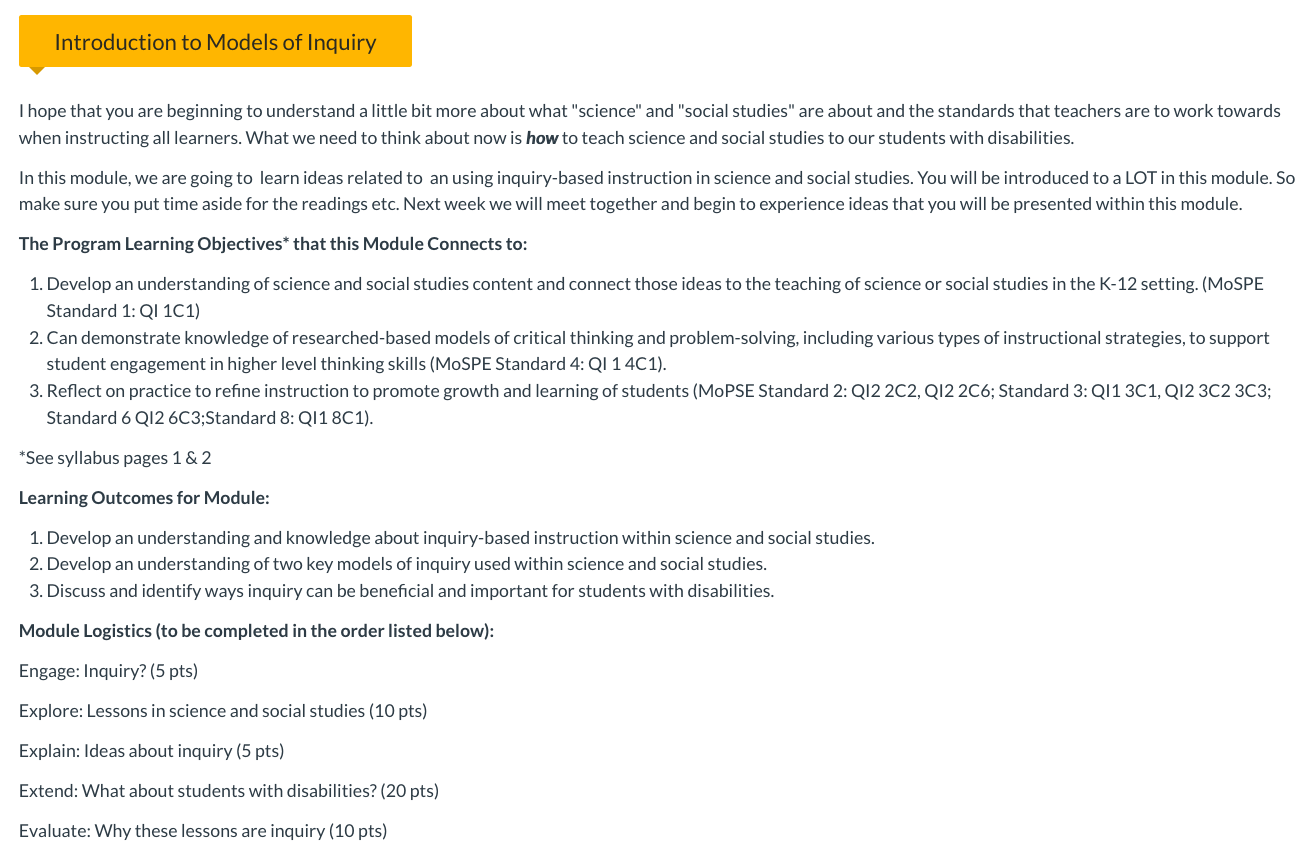
\includegraphics[width=\textwidth]{Fig-1.png}
    \caption{Screenshot of an introduction page to a module.}
\end{figure*}

(transcript of figure 1)

Introduction to Models of Inquiry

I hope that you are beginning to understand a little bit more about what "science" and "social studies" are about and the standards that teachers are to work towards when instructing all learner. What we need to think about now is \textbf{\textit{how}} to teach science and social studies to our students with disabilities.

In this module, we are going to learn ideas related to an using inquiry-based instruction in sscience and social studies. You will be introduced to a LOT in this module. So make sure you put time aside for the readings etc. Next week we will meet together and begin to experience ideas that you will be presented within this module.

\textbf{The program Learning Objectives*} that this Module Connects to:

\begin{enumerate}
    \item Develop an understanding of science and social studies content and connect those ideas to the teaching of science or social studies in the K-12 setting. (MoSPE Standard 1: QI 1C1)
    \item Can demonstrate knowledge of researched-based models of critical thinking and problem-solving, including various types of instructional strategies, to support student engagement in higher level thinking skills (MoSPE Standard 4: QI 1 4C1).
    \item Reflect on practice to refine instruction to promote growth and learning of students (MoPSE Standard 2: QI2 2C2, QI2 2C6: Standard 3: QI1 3C1, QI2 3C2 3C3; Standard 6 QI2 6C3; Standard 8: QI1 8CI).
\end{enumerate}

* See syllabus pages 1 \& 2

\textbf{Learning Outcomes for Module:}

\begin{enumerate}
    \item Develop an understanding and knowledge about inquiry-based instruction within science and social studies.
    \item Develop an understanding of two key models of inquiry used within science and social studies.
    \item Discuss and identify ways inquiry can be beneficial and important for students with disabilities.
\end{enumerate}

\textbf{Module Logistics (to be completed in the order listed below}:

Engage: Inquiry? (5 pts)

Explore: Lessons in science and social studies (10 pts)

Explain: Ideas about inquiry (5 pts)

Extend: What about students with disabilities? (20 pts)

Evaluate: Why these lessons are inquiry (10 pts)

(end transcription)

The course, thus far, has been taught in its current hybrid format twice.  During the first iteration of the course, feedback and data was collected to inform what, if anything, should change the next time it was taught. During the second iteration of the course, there were minor adjustments to the content of the course (e.g., streamlining of content, moving order of topics around, addressing misunderstood content), however, the structure, learning objectives, and major assessment were not adjusted. Because of the sequencing of the special education program, the pre-service teachers were completing their required student teaching competency while they took this course. Although this did cause stress on time and cognitive resources for the pre-service teachers, an advantage was that the course placement did allow the instructors to connect course content to the field placement as a way to apply what was being learned (e.g., informally interviewing teachers to better understand perceptions of those working in the field). 

\begin{table*}[!htbp]
\begin{tabular}{|l|l|l|l|}
\hline
\textbf{5E Phase} & \textbf{Traditional Learning Environment} & \textbf{Online Environment – Modifications} & \textbf{Example Activities in Online Course for Each Phase} \\ \hline
Engage & Students are engaged in situational learning experiences with the intention of sparking curiosity and connecting to background knowledge. In addition, the teacher primes thinking to the new learning concept and determines current knowledge and possible misconceptions. & Focused on a key pedagogical concept(s) as opposed to science concept(s). & \begin{tabular}[x]{@{}l@{}}Cartoon examination \\ Reflection on past situations \\ Watch interesting or thought-provoking video connected to new topic \end{tabular}\\ \hline
Explore	& Exploration allows students to engage in a common activity or group of activities. Here students are solving, questioning, designing and conducting investigations. This allows the teacher to more deeply identify student understanding of the current topic relative to the science curriculum. & The students explored resources that discussed current research and theory connect to key pedagogical concept(s) and collaborate with others to gather ideas.	& \begin{tabular}[x]{@{}l@{}} Observe the way that this instructional skill/strategy is being carried out in field placement \\ Conduct interview to explore current views related to a topic \\ Reflect on practices that the student is engaged in \end{tabular} \\ \hline
Explain	& In this phase, students construct meaning from their experiences in the engage and explore phases. The teacher clarifies concepts, practices, or skills relative to the content. Resources and questions guide learners to form a deeper understanding of science concepts. Oftentimes, knowledge from prior phases is formalized so that it can be clearly articulated and understood by the students. & The students were taught important ideas and themes and had misconceptions clarified. This was often connected to an assignment that required the students to apply their understanding to instructional scenarios and problems in science or social studies that were book based. & \begin{tabular}[x]{@{}l@{}} Read current literature \\ Watch videos by experts in the field \\ Examine lesson plans/case studies that illustrate presented topic \end{tabular} \\ \hline
Extend (or Elaborate) & Activities are presented that challenge and extend students’ understanding and skills to a new context and allows for further practice. Students take their understanding and knowledge from earlier phases and, through a new experience, develop a deeper and broader understanding.	& Students were required to apply the content into to make the abstract, “real-world” and encourage students to try new ideas. & \begin{tabular}[x]{@{}l@{}} Apply new skill(s) to current teaching placement \\ Reflect on how students could use the pedagogical practice and what barriers may exist when implementing \end{tabular} \\ \hline
Evaluate & The evaluation phase allows both students to assess their own understandings, as well as teachers to assess their students. Teachers are determining if students’ skills and understandings are progressing towards the learning outcomes. & Students reflect back, notice pedagogical misconceptions they started with and changed, evaluate their ability to apply concepts and evaluate other’s knowledge to provide meaningful feedback. & \begin{tabular}[x]{@{}l@{}} Reflect on the application of skill(s) in the field \\ Evaluate responses from the engage discussion and refine after completing the learning cycle \end{tabular} \\ \hline
\end{tabular}
\captionof{figure}{5E Instructional Model explanation of phases and how implemented in the online class.}
\end{table*}

\subsection*{5E Instructional Model Modules}

This course relied on the 5E Instructional Model to scaffold the pre-service teacher’s learning each week. The online modules required that the students carry out the learning activities in the order of the model. The majority of the learning activities tied to the instructional model also had a formative assessment embedded so that students were accountable for learning in each section of the module. Each module was comprised of the same 6 components. The first component was a page (see figure 1) with a brief introduction to the module followed by the course objectives to be addressed, specific learning goals for the content, and the logistics of the module (e.g., points per phase). 

The remaining 5 components of the module were each phase of the 5E Instructional Model (Bybee, 2019). Each phase involved a learning activity (or series of activities) and an assignment to submit in response. In Figure 2 we summarize the 5E Instructional Model (Bybee, 2019) and how we enacted it for this course along with sample activities or question stems we used for each phase.

\section*{INSTRUCTORS}

The course has been taught by two instructors. One instructor is a professor in the department of special education. She has been involved in multiple research projects focused on science learning and teaching. The second instructor, at the time, was a third-year doctoral candidate—also from the department of special education—with research interests in Universal Design for Learning and technologies that increase access for all students. The instructors met weekly to discuss the course and create and/or refine modules based on the needs of the pre-service teacher's responses from past lessons. This allowed freedom for the instructors to be responsive to their needs while accomplishing the goals of the class.  

\section*{PRE-SERVICE TEACHERS RESPONSE TO THE 5E INSTRUCTIONAL MODEL}
	
The use of the 5E Instructional Model as a way to structure this course to both convey content and provide experiences in inquiry within a hybrid course, to the best of our knowledge, has not been carried out before. Given the lack of research and the innovative way we used the 5E Instructional Model, we thought it would be important to explore our pre-service teacher’s perceptions of our instructional approach in our most recent iteration of teaching the course to understand if and how the use of the 5E Instructional Model worked and as a way to guide future implementation of the course. The 28 participants in this course were primarily Caucasian females ranging in 21-28 years of age. We collected their perceptions of the course including the use of the 5E Instructional Modal via an end-of-course reflection assignment that involved writing reflective essays for specific question prompts. We employed qualitative analytic techniques (i.e., pattern identification, categorization of quotes, and identification of themes and sub-themes; Creswell \& Poth, 2018) along with individual and team verification processes to ensure that the most accurate picture of student perceptions was identified. Following this analysis, several interesting perceptions emerged. We discuss those next.

\subsection*{``Practicing What We Preach''} 
Methods courses in education have the potential to shape the practice of new teachers (Abell \& Bryan, 1997; Gess-Newsome, 1999). Therefore, in addition to using the 5E Instructional Model within our course as a way to reflect our theoretical orientation to teaching, we sought to model the same type of instruction we expected our pre-service teachers to use with their learners. This approach to learning is something that many of our students would not have experienced as learners. Therefore, as Hanuscin and Lee (2008) note, “Providing opportunities for preservice teachers to experience this approach \textit{as a learner} can be critical to their understanding of the learning cycle” (p. 53). What was exciting to find within the data was that our modeling of the 5E Instructional Model, even within an online format, had a positive impact on the student’s ability to “see” how the model worked and, even more importantly, how they might apply it with their learners. For example, one student wrote, \textit{“We were living out how it is done, as each lesson was set up in a 5E Instructional Model... We were able to see how these concepts looked in real life, as we were actively participating in it.''} 
 
Another student wrote, \textit{``I really loved getting the opportunity to complete 5E on the modules and then also get to see it done in class. That was a huge turning point in the semester and allowed me to really visualize what this should look like in a classroom.”}
This student wrote,
\begin{quote} 
    \textit{“The 5E model allowed for me to experience and engage with the material, which deepened my understanding of the concepts. It also allowed for me to see how 5E, which was a core concept we learned, actually looks like in action. I truly enjoyed this class because I felt that the concepts we were learning were useful and helpful, as seen through our active engagement with them. It was the first time in my college career that I felt like I had a hands-on role in my learning and that I was learning through a process of building off of understanding from prior activities.”}
\end{quote}

Finally, this student wrote, 

\begin{quote}
    \textit{“We were able to see how these concepts looked in real life, as we were actively participating in it. It turned these concepts into a theoretical framework to use in our future classrooms that is proven to work, to actively seeing and benefitting from the positive effects that these frameworks have on student learning. We have clear understandings and personal experiences with the core concepts of this class.”}
\end{quote}

\subsection*{Meaningful and Connected Learning}

There is an increasing amount of online learning delivery that is reshaping the way that learners interact with content and the way that teachers’ structure and communicate their content with students (Allen \& Seamen, 2016; Bates, 2018). A large number of college level classes are now offered via an online platform as opposed to face-to-face. This shift to the online environment can offer instructors affordances for content, delivery, interaction, and new forms of facilitation, however, questions remain as to what “quality” online teaching looks like. Hénard (2010) notes, “In many institutions, quality teaching is a new, but rather vague and often controversial idea” (p. 35).  

Several standards (i.e., National Standards for Online Teaching, Quality Matters Standards) have been developed to help guide instructors to create and deliver quality content via the online learning environment (Banister, Vannatta, \& Ross, 2019; Robinson \& McFadden, 2018). Additionally, research suggests that best practices for offline teaching (e.g., instructor engagement, small class/group size, active learning) can also translate to the online classroom (Brown \& Ayala, 2018; D'Agustino, 2012; Evans, Knight \& Walker, 2019; Lowenthal, Nyland, Jung, Dunlap, \& Kepka, 2019; Martin, Ritzhaupt, Kumar, \& Budhrani, 2019; Sharoff, 2019). Despite the standards and research available to ensure online learning environments are of high quality, there appears to be little guidance available on what structures may promote meaningful and connected learning. From the data we collected, there were three ways that they perceived the 5E Instructional Model to support meaningful learning and engagement in the course. 

First, the structure of the 5E Instructional Model helped students manage their workload over the course of a module. As one student noted, \textit{“I really liked the 5E Instructional Model. I like that the framework was very specific, clear, and easy to follow. It told me exactly what to expect and when to expect it.”} Another student said, \textit{“Having a consistent learning format aided in my learning because I was able to become familiar with the expectations each week.”} Furthermore, as one student wrote, 
\begin{quote}
    \textit{“Another aspect of this} [instructional model] \textit{that I found helpful was that it was broken up into pieces. This helped me to plan out my work because I knew I would do the first two this day and the next three another day or however I chose to break it up. This structure made the modules feel less heavy and overwhelming than they would have felt if I was given a sheet that listed everything I had to do for each module.”}
\end{quote}

Second, the phases of the 5E Instructional Model provided a systematic, exploratory way for students to learn, however, it is important to reiterate that this was accomplished within an online learning format. The following quotes from three students in the course demonstrate this. First, \textit{“The cycle allowed for opportunity to continually dig deeper into the content. Each section of the modules progressively made me think more about the topic.”} And, \textit{“The 5E cycle added to my learning, as it progressively taught and engaged me in the course material… I was able to learn hands-on, which gave me meaningful experiences in the content, and ultimately helped me deeply understand course concepts.”} Finally, \textit{“The 5E model promoted inquiry and student exploration of the content rather than just being told information. This made the content more meaningful and I feel like I learned much more from this design then other class designs I have had.”}

Third, the pre-service teachers recognized that the structure not only expected but promoted reflective thinking on learning and practice.  As one student noted, 

\begin{quote}
    \textit{“Another learning activity that typically deepened my understanding was the reflective writing pieces usually found in the “evaluate” piece of the 5 E learning cycle. These pieces always came at the end of module and they featured questions that were very effective at making me think about the knowledge that I had acquired.”}
\end{quote}

Similarly, this student stated, 

\begin{quote}
    \textit{“I also liked that there was a reflective piece at the end of each module. Whether I was reflecting on the content itself or my own teaching practices, it is something I enjoyed.} Another student stated she … \textit{enjoyed the 5E model because I felt myself reflecting metacognitively about the content for that week throughout the cycle.”} 
\end{quote}

\subsection*{It's for Students with Disabilities Too!}

A fundamental assumption made by instructors in many teacher education pedagogical courses is that what is presented will necessarily be learned and naturally applied outside coursework (Kahn, Pigman, \& Ottley, 2017). Unfortunately, there is research that suggests that informal “on the job training” tends to be the key source for training (e.g., Kahn \& Lewis, 2014) and that many special education teachers feel unprepared to teach content, including science (Irving, Nti, \& Johnson, 2007). Limited research exists on how best to prepare our special education pre-service teachers, but there is research to suggest that good pedagogical practices, such as the 5E Instructional Model, can provide a way for improving instruction (e.g., Brown, Friedrichsen, \& Abell, 2012). A surprising but extremely exciting finding in the data was that not only did students learn from our modeling as seen in the first main theme, they recognized, and in some cases saw, how beneficial this approach could be for students with disabilities. As one student wrote, \textit{“My thinking about inquiry based learning evolved in this class from not knowing how to use inquiry based learning to knowing how to implement it in the classroom for students with disabilities.”} This student wrote,

\begin{quote}
    \textit{“I felt that an inquiry based instructional approach would be largely difficult for students with disabilities including students who struggle with skills such as processing skills, communication and executive functioning. As I reached the Extend portion of Module 2, my knowledge had evolved in understanding the benefits that inquiry based instruction can promote for students with disabilities.”}
\end{quote}

The following two quotes below reflect how some students actually applied what they learned in their current practicum experience. What is important to note is that there was no requirement in the course to apply the 5E Instructional Model, these students, and others, saw to apply it on their own. 

\begin{quote}
    \textit{“After learning about the 5E learning cycle I also began implementing components into my own classroom. I was creating lessons that closely followed the 5E model and encouraged my students to experiment with ideas, ask questions, and draw their own conclusions.”}
\end{quote}
And,
\begin{quote}
    \textit{“The concepts that I found really useful were the models of inquiry... I found these concepts useful because during my student teaching, I noticed I was struggling to keep all students actively engaged in my lessons. These...concepts helped me keep them engaged and understand what barriers were the causes of them not being engaged. Through my use of these concepts, I learned what ways worked for my students to keep them engaged and what didn’t.”}
\end{quote}

\section*{FINAL THOUGHTS AND IMPLICATIONS}

Online learning can lead students to being frustrated and having negative emotions, especially if courses are poorly designed (Kaufman, 2015). Mishra and Koheler (2009) suggest that to develop quality online environments it is important to make solid pedagogical decisions first, then the technological decisions in support of pedagogical decisions. In designing our course, we started with the 5E Instructional Model because we knew it reflected sound pedagogical practice for engaging students in learning with a lens on inquiry. Based on student’s perceptions, the use of the 5E Instructional Model demonstrated to be of benefit to their own learning and pedagogical practice for students with disabilities.  

Although this approach to instruction demonstrates promise, we would be remiss if we did not share two big lessons we learned that need to be considered if using our approach. First, in order to get the students to complete each phase of the Instructional Model within each module and not skip any of the phases, we had to incentivize via points towards their grade, each phase. Consequently, we had 5 rounds of grading per module—along with other assignments assigned. While it is possible to create assignments that require less grading and feedback for “accuracy” and more of a completion of work (e.g., assignments that ask students to recall a situation), there was a lot of grading to manage. To what extent this would work in a larger class setting than ours would need to be investigated. Second, although the consensus was positive towards the course, at times the students felt it was a lot of work. (This was feedback given in general via the assessment module and not connected specifically to the 5E Instructional Model.) Our challenge, especially as we prepare for the next iteration of the course is to find the right balance of work for the special education pre-service teachers to not become overwhelmed and miss an opportunity for meaningful learning whether for themselves or their students with disabilities.

\end{large}
\clearpage 
\section*{REFERENCES}\par 

\leftskip 0.25in
\parindent -0.25in

Abell, S. \& Bryan, L.A., (1997). Reconceptualizing the elementary science methods course using a reflection orientation. \textit{Journal of Science Teacher Education, 8}(3) 153-166.

Abell S. K., Smith D. C., \& Volkmann M. J. (2006). Inquiry in science teacher education. In \textit{Scientific Inquiry and Nature of Science. Science \& Technology Education Library} (pp 173-199), Springer: Dordrecht.

Abell, S. K., \& Volkmann, M. J. (2006). \textit{Seamless assessment in science: A guide for elementary and middle school teachers.} Heinemann/NSTA: Arlington, VA.

Allen, I. E., \& Seamen, J. (2016). \textit{Online report card: Tracking online education in the United States.} Babson Park, MA: Babson Survey Research Group and Quabog Research Group. Retrieved from: \url{https://files.eric.ed.gov/fulltext/ED572777.pdf}

Balci, S., Cakiroglu, J., \& Tekkaya, C. (2006). Engagement, exploration, explanation, extension, and evaluation (5E) learning cycle and conceptual change text as learning tools. \textit{Biochemistry and Molecular Biology Education, 34}(3), 199-203.

Banister, S., Vannatta, R. \& Ross, C. (2019). Piloting a QM-inspired quality assurance process for all online course offerings at a mid-sized university. Proceedings of Society for Information Technology \& Teacher Education International Conference. 380-385.

Bates, A. W. T (2018). \textit{Teaching in a Digital Age: Guidelines for Designing Teaching and Learning.} Retrieved from: \url{https://openlibrary-repo.ecampusontario.ca/jspui/handle/123456789/276}

Bransford J.D., Brown A.L., \& Cocking R. R. (2000). \textit{How People Learn.} Available from: \url{http://www.csun.edu/~SB4310/How\%20People\%20Learn.pdf}

Brown, B., \& Ayala, J. (2018). Themed Conversation: Tips for Active Learning in Online Environments. University of Calgary, Calgary AB. Retrieved from: \url{http://dx.doi.org/10.11575/PRISM/9359}

Brown, P. Friedrichsen, P., \& Abell, S. (2012). The development of prospective secondary biology teachers PCK, \textit{Journal of Science Teacher Education, 23}, 133-155. DOI 10.1007/s10972-012-9312-1

Bybee, R. (2015).  \textit{The BSCS 5E Instructional Model. Creating teachable moments}. Arlington, VA: NSTA Press.

Bybee, R. W. (2019). Using the BSCS 5E Instructional Model to introduce STEM disciplines. \textit{Science and Children, 56}(6), 8-12.

Coulson, D. (2002). \textit{BSCS Science: An inquiry approach-2002 evaluation findings}. Arnold, MD: PS International.

Creswell, J. W., \& Poth, C. N.(2018). \textit{Qualitative inquiry \& research design: Choosing among five approaches} (\nth{4} ed.). Sage.

D'Agustino, S. (2012). Toward a course conversion model for distance learning: A review of best practices. \textit{Journal of International Education in Business, 5}(2), 145-162. Retrieved from: \url{http://dx.doi.org/10.1108/18363261211281753}

Evans, S., Knight, T., Walker, A. \& Sutherland-Smith, W. (2019). Facilitators’ teaching and social presence in online asynchronous interprofessional education discussion. \textit{Journal of Interprofessional Care}. Retrieved from: \url{https://doi.org/10.1080/13561820.2019.1622517}

Gess-Newsome, J. (1999). Pedagogical content knowledge: An introduction and orientation. In \textit{Examining pedagogical content knowledge} (pp. 3-17). Springer, Dordrecht.

Hanuscin, D. L. \& Lee, M. H. (2008)Using the learning cycle as a model for teaching the learning cycle to preservice elementary teachers. \textit{Journal of Elementary Science Education, 20}(2,) 51-66. Retrieved from: \url{https://link.springer.com/content/pdf/10.1007\%2FBF03173670.pdf}

Hénard, F. (2010). Learning our lesson review of quality teaching in higher education: review of quality teaching in higher education. Retrieved from: \url{https://books.google.com/books?hl=en\&lr=\&id=mi7WAgAAQBAJ\&oi=fnd\&pg=PA3\&dq=Hénard,+(2010)+\&ots=ovH\_Lt2idM\&sig=JCUzJw_uIqcS0NIniFrUtZfm87U\#v=onepage\&q=Hénard\%2C\%20(2010)\&f=false}

Irving, M. M., Nti, M., \& Johnson, W. (2007). Meeting the Needs of the Special Learner in Science. \textit{International Journal of Special Education, 22}(3), 109-118.

Kahn, S., \& Lewis, A. R. (2014). Survey on teaching science to K-12 students with disabilities: Teacher preparedness and attitudes. \textit{Journal of Science Teacher Education, 25}(8), 885-910.

Kahn, S., Pigman, R., \& Ottley, J. (2017). A Tale of Two Courses: Exploring Teacher Candidates' Translation of Science and Special Education Methods Instruction into Inclusive Science Practices. \textit{Journal of Science Education for Students with Disabilities, 20}(1), 50-68.

Kauffman, H. (2015). A review of predictive factors of student success in and satisfaction with online learning. \textit{Research in Learning Technology, 23}.

Koehler, M. J., \& Mishra, P. (2009). What is technological pedagogical content knowledge? \textit{Contemporary Issues in Technology and Teacher Education, 9}(1), 60-70.

Lowenthal, P. R., Nyland, R., Jung, E., Dunlap, J. C., \& Kepka, J. (2019). Does class size matter? An exploration into faculty perceptions of teaching high-enrollment online courses. \textit{American Journal of Distance Education, 33}(3), 152-168.

Lunenberg, M., Korthagen, F., \& Swennen, A. (2007). The teacher educator as a role model. \textit{Teaching and Teacher Education, 23}(5), 586-601. 

Marek, E. A., \& Methven, S.B. (1991). Effects of the learning cycle upon student and classroom teacher performance. \textit{Journal of Research in Science Teaching, 28}(1), 41-53.

Martin, F., Budhrani, K., Kumar, S., \& Ritzhaupt, A. (2019). Award-Winning Faculty Online Teaching Practices: Roles and Competencies. \textit{Online Learning, 23}(1), 184-205.

Moore, E. J. \& Bell, S. M. (2019) Is instructor (faculty) modeling an effective practice for teacher education?  Insights and supports for new research. \textit{Action in Teacher Education, 41}(4), 325-343. 

Musheno, B. V. \& Lawson, A. E. (1999). Effects of learning cycle and traditional text on comprehension of science concepts by students at differing reasoning levels. \textit{Journal of Research in Science Teaching, 36}(1), 23–37. 

Nation Council for Accreditation of Teacher Education. (2010). \textit{Transforming teacher education through clinical practice: A national strategy to prepare effective teachers. Report of the blue ribbon panel on clinical preparation and partnerships for improved learning}. Washington, DC: ERIC Clearinghouse.

Robinson, D., \& McFadden, C. (2018). Sexuality in a diverse society: Perspectives on the quality matters/gold review process for online course transition. \textit{International Journal of Technology in Teaching and Learning, 14}(2), 65-80.

Scruggs, T. E., \& Mastropieri, M. A. (2007). Science learning in special education: The case for constructed versus instructed learning. \textit{Exceptionality, 15}(2), 57-74.

Settlage, J. (2000). Understanding the learning cycle: Influences on abilities to embrace the approach by preservice elementary school teachers. \textit{Science Education, 84}, 43-50. 

Sharoff, L. (2019) Creative and innovative online teaching strategies: Facilitation for active anticipation. \textit{Journal of Educators Online, 16}(2). Retrieved from: \url{https://files.eric.ed.gov/fulltext/EJ1223934.pdf}

Taylor, J, Getty, S, Kowalski, C, Wilson, J, Carlson, J, \& Van Scotter, P. (2015). An efficacy trial of research-based curriculum materials with curriculum-based professional development. \textit{American Educational Research Journal, 52}(5) 984-1017.

Taylor, J. C., Therrien, W. J., Kaldenberg, E., Watt, S., Chanlen, N., \& Hand, B. (2012). Using an inquiry-based teaching approach to improve science outcomes for students with disabilities: Snapshot and longitudinal data. \textit{Journal of Science Education for Students with Disabilities, 15}(1), 27-39.

Taylor, J.A., Van Scotter, P., \& Coulson, D. (2007). Bridging research on learning and student achievement: The role of instructional materials. \textit{Science Educator, 16}(2) 44-50.

Therrien, W. J., Taylor, J. C., Hosp, J. L., Kaldenberg, E. R., \& Gorsh, J. (2011). Science instruction for students with learning disabilities: A meta‐analysis. \textit{Learning Disabilities Research \& Practice, 26}(4), 188-203.

Therrien, W. J., Taylor, J. C., Watt, S., \& Kaldenberg, E. R. (2014). Science instruction for students with emotional and behavioral disorders. \textit{Remedial and Special Education, 35}(1), 15-27.

Varma, T., Volkmann, M. \& Hanuscin, D. (2009). Preservice elementary teachers’ perceptions of their understanding of inquiry and inquiry-based science pedagogy: Influence of an elementary science education methods course and a science field experience. \textit{Journal of Elementary Science Education, 21}(1), 1-22. Retrieved from: \url{https://doi.org/10.1007/BF03182354}

Wilson, C., Taylor, J., Kowalski, S., \& Carlson, J. (2010). The relative effects and equity of inquiry-based and commonplace science teaching on students’ knowledge, reasoning, and argumentation. \textit{Journal of Research in Science Teaching, 47}(3), 276 – 301.

\end{document}